%\documentclass[]{article}
\documentclass{scrartcl}
\usepackage{graphicx}
\usepackage[english]{babel}
\usepackage[a4paper]{geometry}
\usepackage{hyperref}
%opening
\title{Distributed Systems: Java RMI session 2/3}
\author{Jago Gyselinck, Armin Halilovic}

\begin{document}
	\maketitle

	\section{Overview}
	Our design consists of three major components: the client(s), the rentalAgency and sessions, and the car rental
	company server(s). A lot of code is inherited from the previous JEE and RMI assignments so responsibilities are similiar.
	
	\textbf{The rental agency} serves as a central hub that the clients communicate with, and serves as a naming server
	        where car rental companies are registered. It also manages the sessions that managers or renters can use.
	        Those sessions can then directly interact with the car rental companies registered with the rental agency.

	\textbf{The client} interacts only with the central rental agency, which serves it sessions it can use to perform
	        the required managerial/reservation tasks in the assignment.

    \textbf{The car rental companies} fulfill their traditional role, they live on separate servers that load their
            respective data files, but aren't adjusted much compared to previous assignments.

    \subsection{Serializable classes}
    The following classes are serializable: 
    \begin{itemize}
    	% CarRentalCompany is enkel remote, niet serializable :) 
		\item \texttt{Car, CarType, Quote, Reservation, ReservationConstraints}
		\item We made these classes serializable as data of their type has to be
		      communicated between different distributed components.
		\item An example of this could be the \texttt{getAvailableCarTypes} method which
		      returns \texttt{Set<CarType>} and is made available in the \texttt{CarRentalCompanyRemote} interface.
		      The class \texttt{ReservationSession} makes use of this method, but resides on a different distributed component.
		      For the method invocation on a remote reference of type \texttt{CarRentalCompanyRemote} to succeed, \texttt{CarType} must be serializable.
	\end{itemize}

    \subsection{Remote classes}
	The following classes are remotely accessible:
	\begin{itemize}
		\item \texttt{CarRentalCompanyRemote, RentalAgencyRemote,\\ ManagerSessionRemote, ReservationSessionRemote}
		\item We made these objects remotely accessible because their
		methods will be invoked from a non-local context, and remote references
		of their type will be passed along between different distributed components.
	\end{itemize}
	
	\subsection{Remote Object Locations}
	\begin{itemize}
		\item Only the sessions (Manager and Reservation) and the Rental Agency
		reside on the same host. This allows the client to request a remote reference
		for the \texttt{CarRentalAgency} via the rmiregistry, and remote references to sessions can
		be requested via that remote reference. Those session remote references are kept in the remote
		\texttt{CarRentalAgency} object so they can be removed later. This organisation also has the
		advantage that when a method is invoked on a \texttt{(Manager/Reservation)Session} through a
		remote reference, the \texttt{CarRentalAgency} it has to interact with is a static object on
		the same component, so no remote interaction is required.
		\item All other remote objects are located on different hosts. The car rental companies each
		reside on their own server as they execute independently of the car rental agency and there can
		be an arbitrary number of them. The client does not interact with them except through the RentalAgency.
		The client is of course also on a separate host, as there too can be as many or as few of them as
		you want, each executing independently and interacting only with the RentalAgency.
	\end{itemize}

	\subsection{Registering of remote objects}
	\begin{itemize}
		\item The \texttt{CarRentalCompanies} and the \texttt{RentalAgency} are registered in
		      the built-in RMI registry. We register the \texttt{RentalAgency} as it is the
		      central starting point for clients to interact with. The \texttt{CarRentalCompanies}
		      are also registered when their respective \texttt{CarRentalServer} starts.
		      Again this is done so that there is some initial reference available that
		      \texttt{ManagerSessions} can use to add the companies to the \texttt{CarRentalAgency}.
		      From then on the \texttt{CarRentalAgency} functions as a \textbf{naming server} for the
		      clients so they can look up \texttt{CarRentalCompanies} by name and not via the rmi registry.
		      The rmi registry offers this functionality too, but would require the client to know the
		      names of the \texttt{CarRentalCompanies} in advance.
		\item \texttt{ManagerSessions} and \texttt{ReservationSessions} are not registered in the
		rmiregistry as they are requested and managed via the \texttt{RentalAgency}.
	\end{itemize}

    \subsection{Life cycle management}
	We were not exactly sure how to handle this at first. During the practical session
	the assistant told us that it was sufficient to implement the methods 
	\texttt{getNewReservationSession} and \texttt{removeReservationSession}.
	The former is called by the client when it wants a remote reference to a
	\texttt{reservationSession}, if a \texttt{reservationSession} already exists for
	the client's name it, then it is returned. Otherwise, it is created. The latter is called by
	the client when they are finished doing their operations and causes the removal of the
	reservationSession coupled to the client's name. \\ This works in a different way for
	\texttt{ManagerSessions}, they are stateless and thus only one \texttt{ManagerSession}
	is kept alive at all times, whose remote reference is returned to serve all managers.

    \subsection{Synchronization}
	We applied synchronization where multiple calls could possibly modify a resource
	concurrently. Examples of this are most of \texttt{ReservationSession}'s methods. 
	This will cause a bottleneck if the application has a lot of concurrent users, but for our testing purposes the difference is not noticeable.
	
	\section{Full class diagram}
    See 'class-diagram.jpg'.

	\section{Deployment diagram}
    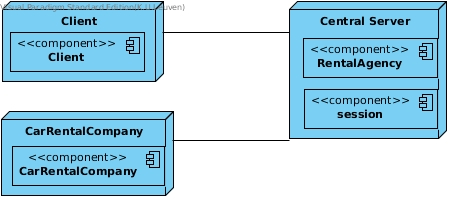
\includegraphics{deployment-diagram.jpg}

    \section{Sequence diagram}
    Sequence diagrams of the booking process have been included in the project.
    See 'sequence-diagram-success.jpg' and 'sequence-diagram-fail.jpg'.

    %    step  | client                     | agency                | crc
    %    1     | getNewReservationSession   | getRentalSession
    %    2.a   | checkForAvailableCarTypes  |                       | getAvailableCarTypes
    %    2.b   | addQuoteToSession(region1)
    %    2.c   | checkForAvailableCarTypes  |                       | getAvailableCarTypes
    %    2.d   | addQuoteToSession(region2)
    %    3     | confirmQuotes
    %    3.a.a |                            | confirmQuotes         | confirmQuote
    %    3.a.b |                            | confirmQuotes         | confirmQuote
    %    4.a   | clearSessions              | removeReservationSession
    %    3.b   |                            | confirmQuotes         | confirmQuote
    %    3.b.a |                            | confirmQuotes         | confirmQuote => ERROR
    %    3.b.c |                            | confirmQuotes         | cancelReservation
    %    4.b.a | throw ReservationException

\end{document}